\subsection{Definition}
\emph{Linear programming} is a method used to determine the optimal solution to a given program. An optimal solution is the best possible outcome achievable under a certain condition.  

It has four key variables. 
\begin{itemize}
\item \textbf{Decision Variable} These variables need to be determined to achieve the optimal solution.
\item \textbf{Objective Function} It's a given function representing the goal to be either maximized or minimized.
\item \textbf{Constrains} These are the conditions that are provided by the use which is expressed as a linear equation or inequality.
\item \textbf{Non-negative restriction} In some cases of investment management and transport problems, the decision variables are required to be non-negative.
\end{itemize}

\subsection{Example of Linear Programming}
Consider Jack's investment portfolio where the decision variables \(x_1\) and \(x_2\) represent the total number of Bitcoins and Dogecoin, respectively, owned by Jack. The price of a single unit of Bitcoin is \(\$7\) and the price of a single unit of Dogecoin is \(\$6\), so the objective function is defined as:

\[
\quad 7x_1 + 6x_2
\]

Jack has the following constraints, probably due to legal/risk issues:

\[
2x_1 + 4x_2 \leq 16 \quad \text{and} \quad 3x_1 + 2x_2 \leq 12.
\]

The constraints can be seen as double the total Bitcoin owned by Jack plus four times the Dogecoin owned by Jack can't exceed 16.

Jack aims to maximize the value of his portfolio by evenly buying Bitcoin and Dogecoin such that his portfolio value is the highest. This scenario has a non-negative constrain that Jack can't own a negative number of Bitcoin or Dogecoin at any time.

With these, the linear program can be defined as the following:
\[
\begin{aligned}
    &\text{Maximize} \quad 7x_1 + 6x_2 \\
    &\text{subject to:} \\
    &\quad 2x_1 + 4x_2 \leq 16, \\
    &\quad 3x_1 + 2x_2 \leq 12, \\
    &\quad x_1, x_2 \geq 0.
\end{aligned}
\]

\subsection{Simplex Algorithm}

One of the ways to solve the optimization problem is using the Simplex Algorithm, which was developed by American mathematician George B. Dantizig. Simplex Algorithm is based on the fundamental theorem of Linear Programming, stated below, but asserts that if an optimal solution exists, it will always occur at one of the corner points (or vertices) of the feasible solution space, which specifically moves from one feasible solution to another, improving the value of the objective function at each step, until the optimal solution is found. The following linear program, one explained above as well, is solved using the Simplex Algorithm.

\subsection{Solving linear program using simplex algorithm}

Consider the following problem, which we will aim to solve using the Simplex Algorithm. \cite{SimplexAlgorithmYouTube}
\[
\begin{aligned}
    &\text{Maximize} \quad 7x_1 + 6x_2 \\
    &\text{subject to:} \\
    &\quad 2x_1 + 4x_2 \leq 16, \\
    &\quad 3x_1 + 2x_2 \leq 12, \\
    &\quad x_1, x_2 \geq 0.
\end{aligned}
\]

\begin{enumerate}
    \item Convert the linear program into standard form by adding the slack variables (i.e., \(s_1, s_2\)). The slack variable is added to remove the inequality sign. 

    \[
    \text{Maximize } 7x_1 + 6x_2
    \]
    \[
    \text{subject to }
    \begin{aligned}
        2x_1 + 4x_2 &\leq 16, \\
        3x_1 + 2x_2 &\leq 12, \\
        x_1, x_2 &\geq 0.
    \end{aligned}
    \]

    And after adding the slack variables.
    
    \[
    \text{Maximize } 7x_1 + 6x_2 + 0s_1 + 0s_2
    \]
    \[
    \text{subject to }
    \begin{aligned}
        2x_1 + 4x_2 + s_1 &= 16, \\
        3x_1 + 2x_2 + s_2 &= 12, \\
        x_1, x_2, s_1, s_2 &\geq 0.
    \end{aligned}
    \]

    \item Develop the initial simplex tableau. The initial Simplex tableau is the first tableau used in the Simplex method that represents the linear programming problem in standard form with the objective function and constraints expressed as equalities. The value in the tableau can be traced back to the maximization equation above after adding the slack variable where the $c_j - z_j$ row holds the coefficients of the objective function whereas the two rows $s_1$ and $s_2$ each hold the co-efficient of the two constrain functions. The $z_j$ column is formed by multiplying the $c_b$ column with the $x_n$ and $s_n$ column. The $c_j$ - $z_j$ is calculated by subtracting the the $z_j$ from $c_b$

    \[
    \begin{array}{cc|cccc|c}
        & & x_1 & x_2 & s_1 & s_2 & \\
        \text{Basis} & c_b & 7  & 6 & 0 & 0 & b\\
        \hline
        s_1 & 0 &  2 & 4 & 1 & 0 & 16 \\
        s_2 & 0 &  3 & 2 & 0 & 1 & 12 \\
        \hline
        & z_j & 0 & 0 & 0 & 0 & 0 \\
        & c_j - z_j & 7 & 6 & 0 & 0  \\
    \end{array}
    \]

    \item Select a non-basic variable with the highest value in \(c_j - z_j\) as the pivot column:

    \[
    \begin{array}{cc|cccc|c}
        & & x_1 & x_2 & s_1 & s_2 & \\
        \text{Basis} & c_b & 7  & 6 & 0 & 0 & b\\
        \hline
        s_1 & 0 &  2 & 4 & 1 & 0 & 16 \\
        s_2 & 0 &  3 & 2 & 0 & 1 & 12 \\
        \hline
        & z_j & 0 & 0 & 0 & 0 & 0 \\
        & c_j - z_j & 7 & 6 & 0 & 0  \\
    \end{array}
    \]

    The pivot column in this case is \(x_1\) since 7 is the highest value in $c_j - z_j$.

    \item Calculate the ratio of \(b\)-column to pivot column values. Select the minimum ratio (pivot row, exiting variable). Once this is selected, the pivot column is replaced by the pivot row. 
 
    \[
    \begin{array}{c|cccc|c|c}
        \text{Basis} & x_1 & x_2 & s_1 & s_2 & b & \text{Ratio} \\
        \hline
        s_1 & 2 & 4 & 1 & 0 & 16 & \frac{16}{2} = 8 \\
        s_2 & 3 & 2 & 0 & 1 & 12 &  \frac{12}{3} = 3\\
    \end{array}
    \]

    Here, the pivot row is \(s_2\) since the $3 < 8$.

    \item Perform elementary row operations to make the pivot column a unit column. Repeat steps 3, 4, and 5 until each \(c_j - z_j \leq 0\).


    \item At the end of the Simplex Algorithm, the following tableau is achieved.

    \[
    \begin{array}{cc|cccc|c}
        & & x_1 & x_2 & s_1 & s_2  \\
        \text{Basis} & c_b & 7  & 6 & 0 & 0 & b\\
        \hline
        x_2 & 6 &  0 & 1 & \frac{3}{8} & -\frac{1}{4} & 3 \\
        x_1 & 7 &  1 & 0 & -\frac{1}{4} & \frac{1}{2} & 2 \\
        \hline
        & z_j & 7 & 6 & \frac{1}{2} & 2 & 32 \\
        & c_j - z_j & 0 & 0 & -\frac{1}{2} & -2  \\
    \end{array}
    \]

    Reading the optimal solution as $x_1$ = 2 and $x_2$ = 3 the objective function is $32$ which can be seen in the $b$ column.
\end{enumerate}


\subsection{How does LP differ from Integer Programming?}

Linear programming (LP) is a mathematical method for formulating an optimization problem in which the objective function and constraints are linear, and the decision variables can take any real value within the feasible region defined by the constraints. In other words, LP assumes that the variables can be fractional.

In contrast, Integer Programming(IP) is a type of optimization problem in which some or all of the decision variables are required to take integer values (whole numbers). IP is classified as a is NP-hard problem. Integer programming is especially useful in problems involving discrete items, such as scheduling problems, knapsack problems, or the maximum matching problem, where the goal is to find the largest matching with discrete pairs. As the name suggests, integer programming can only take integer values.

In a maximum matching problem, the goal is to match items (such as workers to jobs or people to tasks) in such a way that the number of matches is maximized. If fractional matches were allowed, the concept of a match would no longer make sense. Hence, the variables (whether a worker is matched to a job) must take integer values (0 or 1).

\subsection{LP Relaxation}


Since solving the integer program is NP-hard, the integer constraint \( X_e \in \{0, 1\} \) can be relaxed to a continuous constraint \( 0 \leq X_e \leq 1 \), yielding the following LP formulation:

\begin{equation}
    \max \sum_{e \in E} X_e
\end{equation}
subject to:
\begin{equation}
    0 \leq X_e \leq 1, \quad \forall e \in E
\end{equation}
\begin{equation}
    \sum_{e \in \delta(v)} X_e \leq 1, \quad \forall v \in V
\end{equation}


Linear Relaxation helps approximate the solution to the NP-hard problem. By transforming the problem into a Linear Programming Problem, one can leverage the polynomial-time algorithms, like the Simplex Algorithm, to find the solution more efficiently. \cite{fiveable_linear_programming_relaxation}

\subsection{Standard form of Linear Program:}
We say that a linear program is in a standard form if the following are all true: 
\begin{itemize}
\item Non-negative constraints for all decision variables. For instance, $x_1$ and $x_2$ should be positive in the definition example.
\item All remaining constraints should be expressed as equality 
constraints by introducing slack 
variables. 
\item The right-hand side of the constraint function shouldn't be negative.
\end{itemize}

\subsection{Fundamental Theorem of Linear Programming}

Any linear program L, given in standard solution, exactly one of the following holds
\begin{itemize}
    \item has an optimal solution with a finite objective value, 
    \item is infeasible, or
    \item is unbounded
\end{itemize}
    
\subsection{Duality}

One of the key concepts of linear programming is duality which helps us prove the optimality of solutions. The dual of a linear program(the primal) is derived as another linear program (the dual) which involves switching the roles of constraints and variables, turning a maximization problem into a minimization one. The inequalities in the primal become reversed in the dual, and the right-hand side values in the primal become the objective coefficients in the dual. The primal-dual relationship is written below for comparison. \cite{GE}
\[
\begin{array}{rl}
\text{Primal LP:} & \text{Maximize } c^T x \\
                  & \text{subject to } Ax \leq b, \ x \geq 0 \\
\hline
\text{Dual LP:}   & \text{Minimize } b^T y \\
                  & \text{subject to } A^T y \geq c, \ y \geq 0
\end{array}
\]

\subsubsection{Weak Duality Theorem}

The weak Duality Theorem states that for any feasible solutions to the primal and dual, the objective value of the dual is always at least as large as that of the primal. Formally, let \(\bar{x}\) be any feasible solution to the primal and \(\bar{y}\) be any feasible solution to the dual, then:

\[
\sum_{j=1}^n c_j \bar{x}_j \leq \sum_{i=1}^m b_i \bar{y}_i.
\]

This inequality ensures that we can always bound the primal solution from above using the dual solution.

\subsubsection{Strong Duality Theorem}

The strong Duality Theorem states that if the primal problem has an optimal solution, then the dual problem also has an optimal solution, and the objective values of the primal and dual solutions are equal. This is a fundamental result in linear programming and is critical for proving the optimality of the solutions found by the simplex method.

\subsubsection{Example of Strong Duality in the Simplex Algorithm}

Consider the following linear program solved using the Simplex Algorithm.

\[
\text{(Maximize)}: \quad z = 3x_1 + 2x_2
\]
subject to:
\[
x_1 + x_2 \leq 4 \quad 
\]
\[
2x_1 + x_2 \leq 6 \quad 
\]
\[
x_1, x_2 \geq 0
\]
Here the original LP mentioned above is called the Primal Linear Program. We can apply the Simplex Algorithm to find the optimal solution as
\[
x_1 = 2, \quad x_2 = 2, \quad z = 10
\]

Now, the following is the dual of this problem

\[
\text{Dual (Minimize)}: \quad w = 4y_1 + 6y_2
\]
subject to:
\[
y_1 + 2y_2 \geq 3 \quad \text{(dual constraint for } x_1\text{)}
\]
\[
y_1 + y_2 \geq 2 \quad \text{(dual constraint for } x_2\text{)}
\]
\[
y_1, y_2 \geq 0
\]

Solving the dual problem, we find the optimal dual solution to be:
\[
y_1 = 1, \quad y_2 = 1, \quad w = 10
\]

Note that the objective value of the primal (\(z = 9\)) matches the objective value of the dual (\(w = 9\)). This demonstrates \textbf{strong duality}: the optimal values of the primal and dual problems are equal.

The dual of the relaxed LP is closely related to the \textit{Minimum Vertex Cover Problem}. The dual LP is given by:

\begin{equation}
    \min \sum_{v \in V} y_v
\end{equation}
subject to:
\begin{equation}
    y_u + y_v \geq 1, \quad \forall e = (u, v) \in E
\end{equation}
\begin{equation}
    y_v \geq 0, \quad \forall v \in V
\end{equation}


The \emph{Vertex Cover} of a graph is defined as a set of vertices such that at least one endpoint of every edge is included in the set. Mathematically, the vertex cover can be defined as a subset of an original undirected graph \( V \) such that for every edge \( uv \in E \), where E is the set of edges we have \( u \in V' \) or \( v \in V' \), and V' is the set of vertices in the cover graph i.e., every edge has at least one endpoint in the vertex cover \( V' \).
\begin{figure}
    \centering
    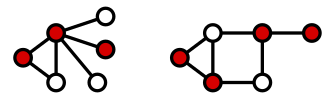
\includegraphics[width=0.5\linewidth]{images/Vertex-cover.svg.png}
    \caption{The figure shows the vertex cover of the two original graphs. The vertices in red are a set of vertex cover. Note that every edge in the graph has at least one endpoint in the vertex cover}
    \label{fig:enter-label}
\end{figure}
The dual of maximum matching problem corresponds to the minimal vertex cover in the graph. \cite{yiu2023research} While the LP solution may give fractional values, for bipartite graphs, the dual LP has an integral solution, as shown in the König's theorem.

\subsection{König's Theorem and its Application}
Kőnig’s Theorem \cite{Konig1916} asserts that in any bipartite graph, the size of the maximum matching equals the size of the minimum vertex cover. 

\begin{proof}[Kőnig's Theorem]
    In any bipartite graph \( G = (U, V, E) \), the size of the maximum matching equals the size of the minimum vertex cover. That is,
    \[
    \text{size(Maximum Matching)} = \text{size(Minimum Vertex Cover)}.
    \]
\end{proof}
